% This must be in the first 5 lines to tell arXiv to use pdfLaTeX, which is strongly recommended.
\pdfoutput=1
% In particular, the hyperref package requires pdfLaTeX in order to break URLs across lines.

\documentclass[11pt]{article}

% Remove the "review" option to generate the final version.
\usepackage[review]{emnlp2021}

% Standard package includes
\usepackage{times}
\usepackage{latexsym}

% For proper rendering and hyphenation of words containing Latin characters (including in bib files)
\usepackage[T1]{fontenc}
% For Vietnamese characters
% \usepackage[T5]{fontenc}
% See https://www.latex-project.org/help/documentation/encguide.pdf for other character sets

% This assumes your files are encoded as UTF8
\usepackage[utf8]{inputenc}

% This is not strictly necessary, and may be commented out,
% but it will improve the layout of the manuscript,
% and will typically save some space.
\usepackage{microtype}
\usepackage{amsmath, amsfonts}
\usepackage{color}
\usepackage{graphicx}
\usepackage{tikz}
\usetikzlibrary{3d}
\usetikzlibrary{arrows.meta}
\usetikzlibrary{backgrounds}
\usetikzlibrary{bayesnet}
\usetikzlibrary{calc}
\usetikzlibrary{calligraphy}
\usetikzlibrary{fit}
\usetikzlibrary{positioning}
\usetikzlibrary{decorations.markings}
\usetikzlibrary{decorations.pathreplacing}
\usetikzlibrary{shapes}
\usetikzlibrary{shapes.geometric}
\usetikzlibrary{shapes.multipart}
\usetikzlibrary{tikzmark}
\usetikzlibrary{shapes}
\usetikzlibrary{shapes.geometric}
\usepackage{xspace}


\graphicspath{{images/}}
\DeclareGraphicsExtensions{.jpg,.png,.pdf}

\newcommand{\TODO}{\textcolor{red}{TODO}\xspace}
\newcommand\todo[1]{\textcolor{red}{#1}}
\newcommand{\ie}{i.e.,\xspace}

\usepackage{cleveref}
\usepackage{tabularx, booktabs}

% If the title and author information does not fit in the area allocated, uncomment the following
%
%\setlength\titlebox{<dim>}
%
% and set <dim> to something 5cm or larger.

\title{Learning Compositional Forms for Grounded Instructions}

% Author information can be set in various styles:
% For several authors from the same institution:
% \author{Author 1 \and ... \and Author n \\
%         Address line \\ ... \\ Address line}
% if the names do not fit well on one line use
%         Author 1 \\ {\bf Author 2} \\ ... \\ {\bf Author n} \\
% For authors from different institutions:
% \author{Author 1 \\ Address line \\  ... \\ Address line
%         \And  ... \And
%         Author n \\ Address line \\ ... \\ Address line}
% To start a seperate ``row'' of authors use \AND, as in
% \author{Author 1 \\ Address line \\  ... \\ Address line
%         \AND
%         Author 2 \\ Address line \\ ... \\ Address line \And
%         Author 3 \\ Address line \\ ... \\ Address line}

\author{First Author \\
  Affiliation / Address line 1 \\
  Affiliation / Address line 2 \\
  Affiliation / Address line 3 \\
  \texttt{email@domain} \\\And
  Second Author \\
  Affiliation / Address line 1 \\
  Affiliation / Address line 2 \\
  Affiliation / Address line 3 \\
  \texttt{email@domain} \\}

\begin{document}
\maketitle
\begin{abstract}
We leverage advances in pre-trained language models to make advances in planning conditioned on language.
\end{abstract}

\section{Introduction}
Inspired by \cite{Lu2019ViLBERTPT} we devise a pre-training task that encourages our model to attend to the instruction and the environment jointly. 
%
At pre-training, the model receives the command and a representation of the initial environment. 
%
The model predicts whether a given command is relevant to the environment.
%
These embeddings will be used downstream by a planner (Section \ref{transformer-planner}) that will be trained to execute natural language structurions.
%
The hope is that these ``grounded'' embeddings will give our planner a head start in learning how the meaning of words can be composed.
%
One imagines that such a joint embedding will be helpful since knowing how to pick out the ``red'' items and the ``square''  items on a grid will be useful in picking out the ``red squares'', even if the phrase has never been seen before.

We will use the grounded-SCAN dataset \cite{ruis2020benchmark} which contains synthetic sentences paired with demonstrations in a grid world.
%
The sentences in the dataset are split so as to test the ability of a model to perform zero-shot generalization.
%
For example, the phrases ``red'', ``blue'', and ``blue square'' all appear in the training data, but the phrase ``red square'' appears only at test-time.

\section{Pre-training to improve grounding}

\subsection*{Multi-modal Entailment Prediction}
\todo{incomplete}
%
We present the model with a sentence and two frames of a demonstration and ask the model to determine if the frames match the sentence.

\subsection{Multi-modal masked language modeling}
\todo{incomplete}
%
In the second masked language modeling task, we mask parts of the image as well as words of the sentence, and ask the model to fill in the missing words.

\section{Naturalistic data}

The data from \citet{ruis2020benchmark} consists of synthetic sentences paired with demonstrations of the sentences being acted out in a grid world.
%
In order to test whether our model is capable of handling naturalistic language, we collected human-generated annotations via Amazon Mechanical Turk.
%
Workers were shown the demonstration video and asked to write the sentence that might have produced the actions shown.
%
In order to push volunteers towards the desired content, we will specify a few dimensions that should be used in the description.
%
In order to preserve the compositional split, we also specified, per example, which properties of an object should not be mentioned.
%
Note that these sentences are to be used at test-time only.
%
Our experiment is to measure the performance of a model, trained on synthetic data, on naturalistic test data.
%
We hope to determine whether the performance of our model is due mostly to the synthetic nature of the data, or if our model is truly capable of handling compositionality, as it is exhibited in human-generated language. 

\section{Multi-modal transformer baseline}
\label{transformer-planner}
\todo{incomplete}
We present our own simple planner to see if we can improve on the baseline given in \cite{ruis2020benchmark}.

\section{Related Work}
\subsection{Visual Language Navigation}
Our setting is very similar to the problem of Visual-Language-Navigation (VLN). 
%
In a VLN task, a robotic agent is given natural language directions to a specified goal location. 
%
The agent must navigate the environment until it reaches the goal.
%
With the advent of Transformers, many approaches have sought to build models for Visual-Language-Navigation \citep{magassouba2021crossmap, fang2019scene, Chen2020TopologicalPW}.
%
The problem that we focus on in this work is strictly more challenging than the VLN task. 
%
Not only must our agent learn to navigate, it must also learn to interact with the objects in the environment according to their attributes.

%
Our work is most related to the approach of \citet{Hao2020TowardsLA}, who present pre-training scheme to create embeddings for use in downstream Visual-Language-Navigation tasks.
%
But, their pre-training scheme relies on predicting an action for a given environment and instruction.
%
Our approach only relies on aligning commands to environments in which they are relevant, which is much less laborious to annotate.
%

\subsection{Transformers for Vision}
Our model takes both language and visual features as input, and thus builds on the work of \citep{LuViLBERT2019, tan-bansal-2019-lxmert, LiVisualBert2019}.

\subsection{Compositional Generalization}
The paper \citep{ruis2020benchmark} that introduced gSCAN also presented a simple baseline model.
%
Since then, numerous improvements on that model have been made \citep{gao-etal-2020-systematic, heinze-think-2020, kuo2020compositional}.
%
However, none of these improvements make use of recent advances in pre-trained language models. 

\section{Data}
Our model is trained on the grounded SCAN benchmark \citep{ruis2020benchmark}, a dataset of synthetic sentences in English paired with demonstrations in a grid world that systematically tests generalizations.
%
We collect a new dataset, grounded SCAN Human (\TODO name), which augments the demonstrations with human generated sentences.
%


\section{Model Architecture}
The training data $D=\{(\mathbf{x}_i, E_i) \}_{i=1}^{i=|D|}$ consists of natural language commands $\mathbf{x}$ paired with an execution $E$. 
%
Each execution $E$ is a tuple of a sequence, $\mathbf{a}$, with $T$ actions and a sequence, $\mathbf{e}$, with $T+1$ environments, where action $\mathbf{a}_t$ results in state  $\mathbf{e}_{t+1}$. 
%
Each environment is represented by $m$ image patches: $\mathbf{e}_{t} = [e_{t,0}\cdots e_{t,m}]$.
%

\Cref{fig:training_model} shows our model as it makes a forward pass during training.
%
Consider an input command $\mathbf{x}_{i}$ of length $n$.
%
At each time-step $t$, the model receives patches $\mathbf{e}_t$ which represent the environment as it appears in that moment. 
%
The command and patches are embedded using a text and vision embedding layer, respectively. 
%
The embeddings are passed to stacked co-transformer and transformer layers, which alternately attend to one and both input modalities.
%
Each co-Transformer also attends to the top-most hidden state representations of the previous time-step.
%
(\todo{TODO: does each co-Transformer in the stack attend to the same hidden states, or only the bottom layer?})
%
The topmost of the stacked transformers outputs a representation of the text as a sequence of $n$ hidden states, $[h_{[CLS]}^l,\cdots,h_{n}^l]$, and a representation of the image patches as $m$ hidden states $[h^e_{[CLS]}, \cdots, h^{e}_{m}]$.
%
A context vector $c_t$ is formed by concatenating $h_{[CLS]}^l$ and $h_{[CLS]}^e$.
%
The context vector passes through a linear projection layer and Softmax, producing a distribution over actions, from which $a_t$ is selected.
%
Decoding precedes auto-regressively.

\begin{figure}
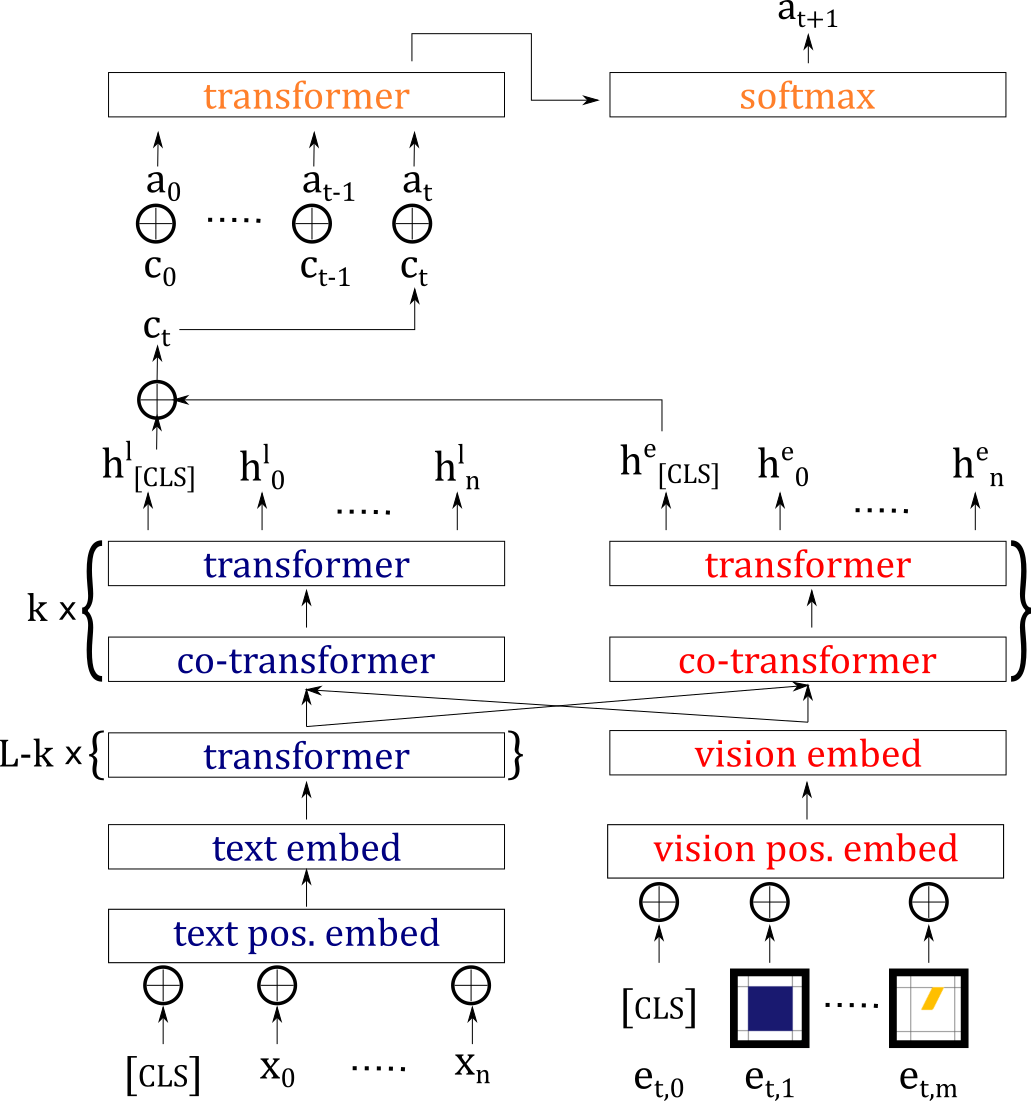
\includegraphics[width=3in]{training_model.png}
\caption{Predicting an action at time $t$. Our model consists of a text encoder (blue), a vision encoder (red), and an action decoder (orange). }
\label{fig:training_model}	
\end{figure}

\subsection{Cross-Attention}
A Transformer layer takes an input sequence of vectors $\mathbf{Q}$, called the query vectors. 
%
For each $q\in \mathbf{Q}$, a context vector is created from a weighted sum of vectors $\mathbf{V}$, called the value vectors.
%
The weights in this sum are generated by taking the dot product between $\mathbf{Q}$ and $\mathbf{K}$, where $\mathbf{K}$ is the set of key vectors that represent $\mathbf{V}$.

In cross-attention, the language co-Transformer takes $\mathbf{Q}_{l}$, $\mathbf{V}_{v}$, $\mathbf{K}_{v}$ as input, where $\mathbf{Q}_l$ are the hidden states of the text Transformer, and $\mathbf{K}_{v}$ and $\mathbf{V}_{v}$ are the hidden states of the vision Transformer.

\section{RNN baseline}
We compare our model with an RNN decoder to show the effectiveness (1) of our pre-training scheme and (2) of our Transformer-based action decoder.
%

We run two experiments.
%
In the first experiment, we first pre-trained our text and vision encoder using grounded masked language modeling. 
%
In the second experiment, we instead use randomly initialized weights for our text and vision encoder.

%
At inference time, the model receives the text and vision encoder create text embeddings, $[h_{[CLS]}^{l},...,h_{n}^{l}]$, for the input command and vision embeddings, $[h_{[CLS]}^{v},...,h_{m}^{v}]$ for the patches for the initial grid.
%
At each time-step $t$, the RNN receives these embeddings, as well as the image features of the environment at that time-step $e_t$.
%
A context vector $c_t$ is created by applying attention to the input embeddings, using the prior hidden state $h_{t-1}$ as the query vector:
\begin{align*}
c_{t,v} &= \text{Attn}_v(h_{t-1}, [h_{[CLS]}^{v},...,h_{m}^{v}])\\
c_{t,l} &= \text{Attn}_l(h_{t-1}, [h_{[CLS]}^{l},...,h_{n}^{l}])\\
c_t &= c_{t,v} + c_{t,l}
\end{align*}
Given this context vector and the previous hidden state $h_{t}$ as input, the RNN produces a new hidden state $h_{t+1}$:
$$
h_{t+1} = RNN(h_t, c_t)
$$
The hidden state at time $t$, $h_t$ is fed through a fully-connected layer, and a softmax is used to produce a distribution over actions, from which the action $a_t$ is sampled:
$$
p(a_{t+1} \mid a_{0:t}, e_{0:t}, x) = \text{Softmax}(FC(h_{t+1}))
$$
%

\Cref{tab:baseline_results} shows the performance of our baseline.

\begin{table*}
\begin{center}
\begin{tabularx}{\textwidth}{ l|ccccc }
\toprule
\multicolumn{1}{c}{} 
& \multicolumn{2}{c}{w/ pre-training}  
& \multicolumn{2}{c}{random}
& \multicolumn{1}{c}{\cite{ruis2020benchmark}}\\
A: Random & test  & val  & test &  val & test \\
\midrule
A: Random & --  & --  & -- &  -- & 97.69 $\pm$ 0.22\\
B: Yellow Squares & --  & --  & -- &  -- & 54.96 $\pm$ 39.39\\
C: Red Squares & --  & --  & -- &  -- & 23.51 $\pm$ 21.82\\
D: Novel Direction & --  & --  & -- &  & 0.00 $\pm$ 0.00 \\
E: Relativity & --  & --  & -- & & 35.02 $\pm$ 2.35 \\
F: Class Inference & --  & --  & -- &  -- & 92.52 $\pm$ 6.75 \\
\bottomrule
\end{tabularx}
\end{center}
\caption{The performance of an RNN decoder using our pre-trained text-environment embeddings vs. using randomly initialized embeddings.}
\label{tab:baseline_results}
\end{table*}

\subsection{Results}

\subsection{Discussion}



% Entries for the entire Anthology, followed by custom entries
\bibliography{anthology,custom}
\bibliographystyle{acl_natbib}

\appendix

\section{Example Appendix}
\label{sec:appendix}

This is an appendix.

\end{document}
